\documentclass[border=0.125cm]{standalone}
\usepackage{tikz}
\usetikzlibrary{positioning}
\usepackage{ifthen}
\usetikzlibrary{matrix,arrows.meta,quotes,shadows,decorations.pathreplacing,positioning,fadings}
\usepackage{cfr-lm}
\usepackage{graphicx}
\usetikzlibrary{shapes,shadows,arrows,positioning,graphs}


\colorlet{mewnol}{blue!75!cyan}%
\colorlet{allanol}{blue!50!black}%

\begin{document}

\tikzset{%
  every neuron/.style={
    circle,
    draw,
    minimum size=1cm
  },
  neuron missing/.style={
    draw=none, 
    scale=4,
    text height=0.333cm,
    execute at begin node=\color{black}$\vdots$
  },
}

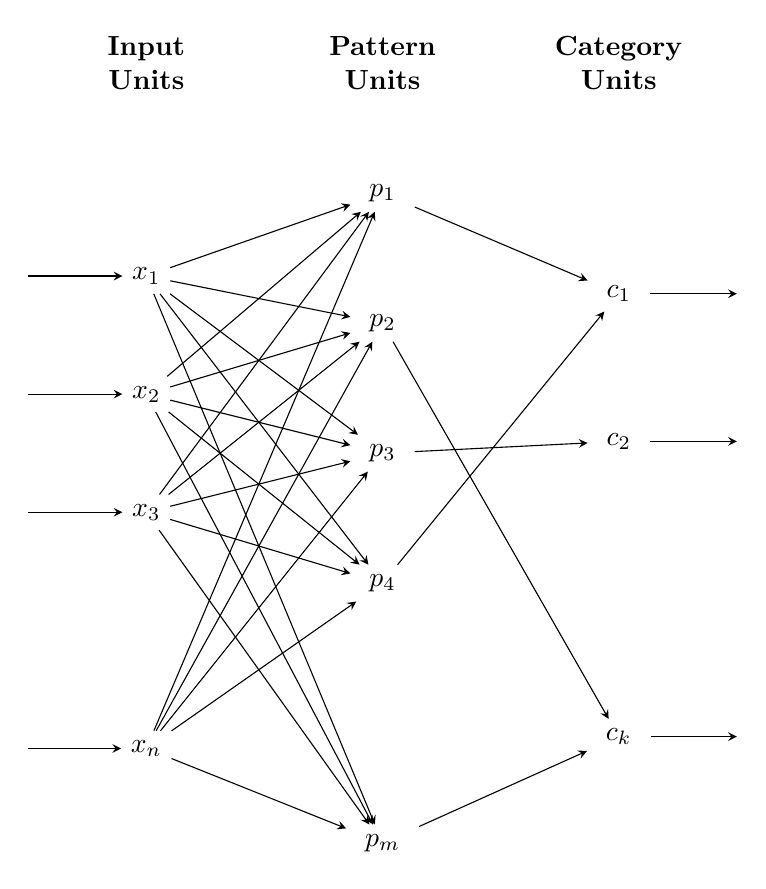
\begin{tikzpicture}[x=1.5cm, y=1.5cm, >=stealth]

\foreach \m/\l [count=\y] in {1,2,3,missing,4}
  \node [every neuron/.try, neuron \m/.try] (input-\m) at (0,2.5-\y) {\ifthenelse{\equal{\m}{missing}}{}{\ifthenelse{\equal{\m}{4}}{$x_n$}{$x_\m$}} };

\foreach \m [count=\y] in {1,2,3,4,missing,5}
  \node [every neuron/.try, neuron \m/.try ] (hidden-\m) at (2,3.3-\y*1.10) 
  {
  	\ifthenelse{\equal{\m}{missing}}{}{
  		\ifthenelse{\equal{\m}{5}}{$p_m$}{$p_\m$}
  	}
  };

\foreach \m [count=\y] in {1,2,missing,3}
  \node [every neuron/.try, neuron \m/.try ] (output-\m) at (4,2.6-\y*1.25) 
  {
  	\ifthenelse{\equal{\m}{missing}}{}{
  		\ifthenelse{\equal{\m}{3}}{$c_k$}{$c_\m$}
  	}
  };

\foreach \l [count=\i] in {1,2,3,n}
  \draw [<-] (input-\i) -- ++(-1,0)
    node [above, midway] {};

\foreach \l [count=\i] in {1,h}
  \node [above] at (hidden-\i.north) {};

\foreach \l [count=\i] in {1,2,3}
  \draw [->] (output-\i) -- ++(1,0)
    node [above, midway] {};

\foreach \i in {1,...,4}
  \foreach \j in {1,...,5}
    \draw [->] (input-\i) -- (hidden-\j);

\foreach \i in {1,4}
	\foreach \j in {1}
    \draw [->] (hidden-\i) -- (output-\j);
    
\foreach \i in {3}
	\foreach \j in {2}
		\draw [->] (hidden-\i) -- (output-\j);
		
\foreach \i in {2,5}
	\foreach \j in {3}
		\draw [->] (hidden-\i) -- (output-\j);

  \node [align=center, above] at (0,3) {\textbf{Input} \\ \textbf{Units}};
  \node [align=center, above] at (2,3) {\textbf{Pattern} \\ \textbf{Units}};
  \node [align=center, above] at (4,3) {\textbf{Category} \\ \textbf{Units}};
 	
\end{tikzpicture}

\end{document}